\chapter{Background}
\label{background}

In this chapter, we provide some background on topics, closely related to this thesis.
In the first section, we explain for which kind of data types hierarchical clustering could be applied. 
We describe the motivation behind them and their purpose. 
In the second part, we examine different types of hierarchical clustering algorithms.

\section{Data structures}
There are numerous ways to categorize data in clustering problems. 
The most frequent definitions are: numerical, categorical, spatial, multivariate, and mixed. 
Depending on data type, different clustering algorithms are used. 
Besides the nature of data, there are different ways to represent the same data types. 
In this work, we consider data being represented as graphs or vectors.

\subsection{Graphs}
\begin{figure}[t]
    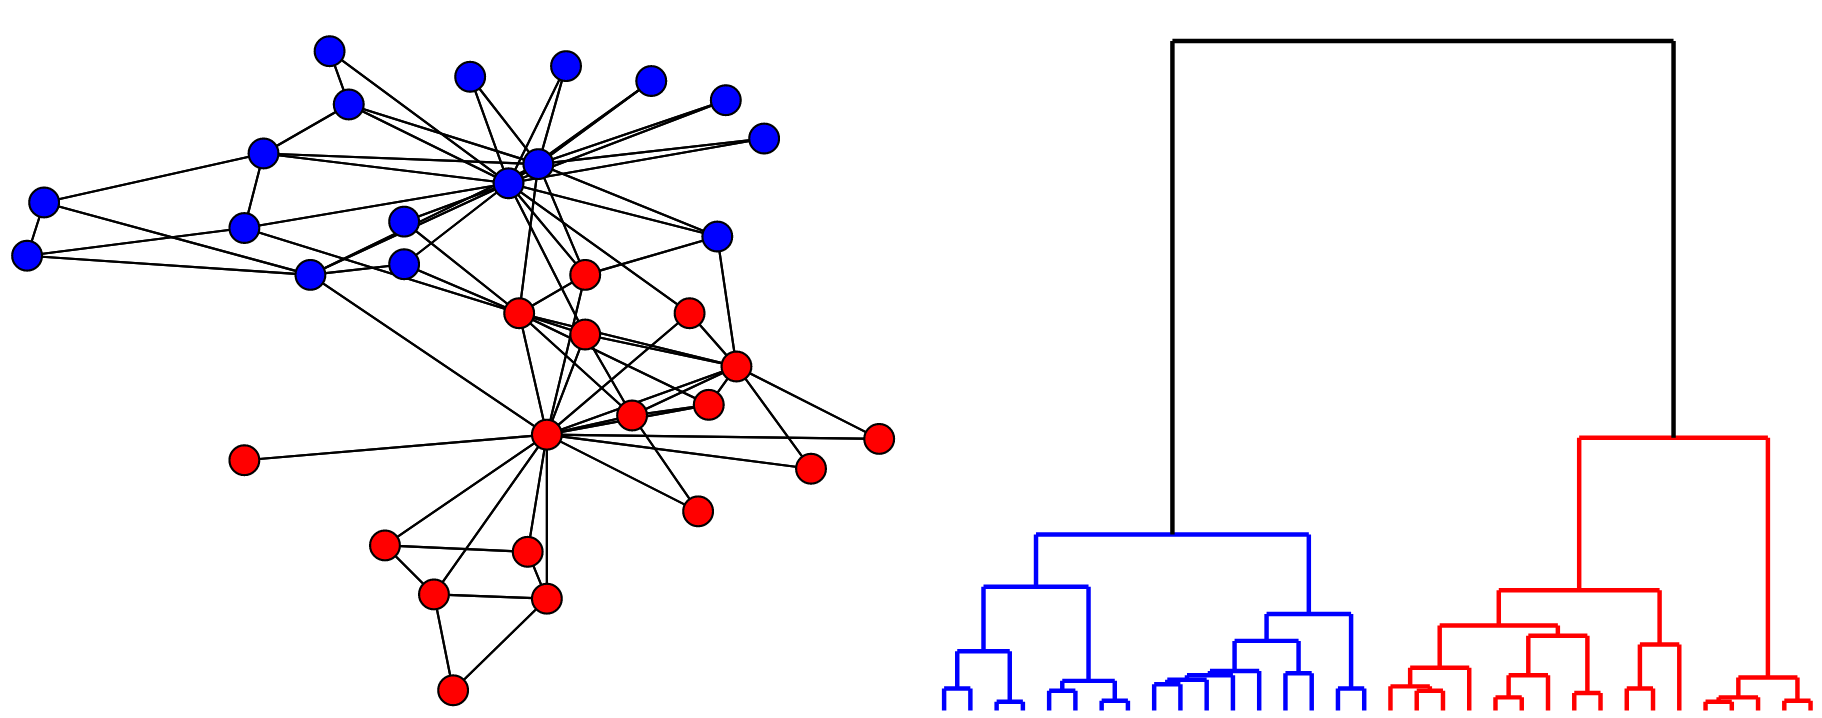
\includegraphics[width=0.8\textwidth,keepaspectratio=true]{figures/Karate_club.png} 
    \centering
    \caption{Graph and its representation as a dendrogram.}
    \label{fig:graph_example}
\end{figure}

Here we display a typical example of an input to hierarchical clustering algorithm - graph, see the Figure \ref{fig:graph_example}: 
directed, undirected or bipartite represented as an adjacency matrix. If the graph is directed, 
then matrix $A$ is symmetric, if the graph is weighted, then $A_{ij}$ represents the weight between edge i and j. 
$V$ describes the set of $n$ vertices or nodes, and $E$ describes the set of $m$ edges \cite{Bonald2018}.

Given a weighted, undirected, connected graph $G = (V, E)$ of $n$ nodes and $m$ edges without self-loops represented as adjacency matrix $A$. We denote by $d=A \mult 1$ the vector of degrees and by $v$ the volume of the graph: $$v=\sum_{i \in V}d_i=\sum_{i,j \in V }A_{ij}$$.

We introduce the definition of \textbf{sampling}. Under edge sampling, each node pair $i$, $j$ is sampled with probability: $$p(i,j)=\frac{A_{i,j}}{v}$$ 
The marginal distribution is calculated as: $$p(i)=\sum_{j \in V}p(i,j)=\frac{d_i}{v}$$ 
If the sampling of node $i$ is known, to calculate the probability of node $j$ is possible through a conditional probability: $$p(j|i)=\frac{p(i,j)}{p(i)}=\frac{A_ij}{d_i}$$

A number of hierarchical clustering algorithms have been developed specifically for graphs \cite{Newman} \cite{Bonald2018} \cite{Newman_2004} \cite{Pascal2005} \cite{Tremblay2014}.

\subsection{Vector Data}
It is probably the most common to represent data. Usually, clustering techniques are applied to vector data. Several clustering algorithms have specifically been developed for this task, they do not directly apply to graphs 
unless the graph is embedded in some metric space. It is possible to transform vector data in graphs and vice versa. The choice of a distance is important for vector data. Common hierarchical clustering techniques are the linkage algorithm with different distance update formula and the nearest-neighbour clustering algorithm \cite{Ward1963HierarchicalGT} \cite{müllner2011modern}.

\section{Hierarchical clustering}
Let's consider $n$ points $x_1, \dots, x_n \in {R}^{d}$, which we would like to cluster in hierarchical way that should capture the natural structure of a real dataset.

\subsection{Divisive approach}
The first class of algorithms to consider is \textit{divisive}, which is a top-down method in which we begin from a single cluster and divide it sequentially before all objects are isolated or other stop criteria are used.
Since there are $\mathcal{O}(2^n)$ ways to break each cluster, the solution is computationally costly.
Therefore, all experiments in this work are conducted using \textit{agglomerative algorithms}.

\subsection{Agglomerative approach}
\label{clustering_algorithms}
In contrast to Divisive, the agglomerative method begins at individual clusters with one data point and merges clusters recursively. The \textit{closest} clusters are merged depending on a distance $d$ between them. The distance $d$ is not necessarily a metric. It is only necessary that $d$ be non-negative and symmetric. The algorithm is the following \cite{Bonald2019notes}:

\begin{enumerate}
    \item Initialization: $K \leftarrow \{\{1\}, \dots, \{n\}\}$
    \item Agglomeration: For $t=1, \dots, n-1$,
        \begin{itemize}
            \item $A,B \leftarrow argmin_{a,b \in K, a \ne b}d(a,b)$
            \item $C \leftarrow A \cup B$ 
            \item $K \leftarrow K \setminus \{A,B\}$
            \item $K \leftarrow K \cup \{C\}$
            \item Output $A,B, d(A,B)$
        \end{itemize}
\end{enumerate}


\paragraph{Ward} 
Ward's distance \cite{Ward1963} is a common distance for Agglomerative algorithms.
Ward seeks to reduce the number of squared disparities in all clusters. It is analogous to the objective function of K-means \cite{Macqueen67somemethods}. Let $g(c)$ be the centroid of any cluster $c$ $$g(c)=\frac{1}{|c|}\sum_{i \in c}x_i$$, and $S$ be the complete square Euclidean distance of points in $c$ to their centroid $$ S(c) = \sum_{i \in c}||x_i - g(c) ||^2$$

Then, after some simplification, we define the distance as: $$d(a,b)= S(a \cup b) - S(a) - S(b)=\frac{|a||b|}{|a|+|b|}||g(a)-g(b)||^2$$

\paragraph{Paris} 
It is a new algorithm for graphs proposed by \cite{Bonald2018}. The choice of “proximity” between nodes follows from sampling. Node $j$ is close to node $i$ if the probability of sampling node $j$ given the sampling of node $i$ is much higher than the probability of sampling node $j$. Hence, similarity between nodes can be expressed as: $$\sigma(i,j)=\frac{p(j|i)}{p(j)}=\frac{p(i,j)}{p(i)p(j)}=v\frac{A_{ij}}{d_i d_j} $$

The general idea of Paris algorithm is:

\begin{algorithm}[h]
    \SetAlgoLined
    \KwIn{G=(V,E)}
    \KwOut{List of merges, $L$}
    \For{$t = 1, \dots , n-1$} {
        $i,j \leftarrow argmax_{i,j \in V, i \ne j}\sigma(i,j)$ \;
        append $i,j$ to $L$
        merge $i,j$ into node $n+t$
        update $\sigma$
    }
    \EndFor
    \caption{Paris algorithm.}
    \label{paris}
\end{algorithm}

\paragraph{Louvain}

\begin{algorithm}[h]
	\SetAlgoLined
	\KwIn{G=(V,E)}
	\KwOut{List of merges}
	
	$clusters \leftarrow Louvain(G)$\;
	\If{$\mid clusters \mid > 1$}{
		$graphs \leftarrow GetSubgraphs(G, clusters)$ \;
		return [$HierarchicalLouvain(S)$ for $S$ in graphs]
	}
	\Else{
		return $[nodes(G)]$
	}
	\caption{Hierarchical Louvain algorithm.}
	\label{HierarchicalLouvain}
\end{algorithm}

Let us now look for the algorithm which uses a modularity as a distance metric. Let $\delta_{C}(i, j) = 1$ if $i$, $j$ are in the same cluster and 0 otherwise. The modularity of clustering $C$ is defined by \cite{Newman_2004}: $$Q(C)=\sum_{i,j \in V}(p(i,j)-p(i)p(j))\delta_{C}(i, j)$$ As a consequence, modularity can be defined as the difference in the probabilities of sampling two nodes from the same cluster using the joint distribution $p(i, j)$ and product $p(i)p(j)$. The Louvain algorithm is composed of 4 steps:

\begin{enumerate}
    \item \textbf{Initialization:} $C \leftarrow \{\{1\}, \dots \{n\}\}$
    \item \textbf{Iteration:} when modularity $Q(C)$ increases, update $C$ by moving one node from one cluster to another.
    \item \textbf{Aggregation:} merge all nodes belonging to the same cluster, update the weights and apply step 2.
    \item Return $C$. 
\end{enumerate}

It is easy to move from the general version of the Louvain clustering algorithm to the hierarchical one, as shown in Algorithm \ref{HierarchicalLouvain}.

\subsection{Dendrograms} 

Regardless of which approach we choose to produce a hierarchical clustering, as an output, we will have a dendrogram Figure \ref{fig:graph_example} as an output. The dendrogram $D$ contains the pair of nodes merged through the run of the algorithm. By browsing the final dendrogram bottom-up, all partitions $P_0, \dots, P_{n-1}$ can be retrieved.
It is worth noting that the partition $P_t$ is made of $n - t$ clusters. Additionally, a dendrogram includes the distance $d_t = d(i, j)$ and number of nodes within $n_{n+t} = n_i + n_j$ a cluster. Each branch is plotted at height $d_t$, thus all distances must be non-decreasing.

\subsection{Trees}
Once we obtain a dendrogram $D$, the next step is to analyze and work with it. A dendrogram's data structure is quite difficult to manage and has no convenient algorithms for it. However, dendrogram could be easily converted into a tree data structure. Formally, a tree is an acyclic and connected graph: $T=(V, E)$ with a set of vertices $V$ and a set of edges $E$. Each node in a tree has zero or more child nodes, which lay under it in the tree. In this work, we mostly study rooted trees. Yet, it is possible to apply a new metric - explained in Chapter \ref{design} - to unrooted trees as well. We store trees in a Newick format \cite{newick1990} which is a very flexible data representation. Therefore, we are going to use terms of dendrograms and trees interchangeably, assuming that we are able to very easily convert dendrograms to trees and backward. 